%%%%%%%%%%%%%%%%%%%%%%%%%%%%%%%%%%%%%%%%%
% University Assignment Title Page 
% LaTeX Template
% Version 1.0 (27/12/12)
%
% This template has been downloaded from:
% http://www.LaTeXTemplates.com
%
% Original author:
% WikiBooks (http://en.wikibooks.org/wiki/LaTeX/Title_Creation)
%
% License:
% CC BY-NC-SA 3.0 (http://creativecommons.org/licenses/by-nc-sa/3.0/)
% 
% Instructions for using this template:
% This title page is capable of being compiled as is. This is not useful for 
% including it in another document. To do this, you have two options: 
%
% 1) Copy/paste everything between \begin{document} and \end{document} 
% starting at \begin{titlepage} and paste this into another LaTeX file where you 
% want your title page.
% OR
% 2) Remove everything outside the \begin{titlepage} and \end{titlepage} and 
% move this file to the same directory as the LaTeX file you wish to add it to. 
% Then add \input{./title_page_1.tex} to your LaTeX file where you want your
% title page.
%
%%%%%%%%%%%%%%%%%%%%%%%%%%%%%%%%%%%%%%%%%
%\title{Title page with logo}
%----------------------------------------------------------------------------------------
%	PACKAGES AND OTHER DOCUMENT CONFIGURATIONS
%----------------------------------------------------------------------------------------

\documentclass[12pt]{article}
\usepackage[english]{babel}
\usepackage[utf8x]{inputenc}
\usepackage{amsmath}
\usepackage{graphicx}
\usepackage[colorinlistoftodos]{todonotes}

\begin{document}

\begin{titlepage}

\newcommand{\HRule}{\rule{\linewidth}{0.5mm}} % Defines a new command for the horizontal lines, change thickness here

\center % Center everything on the page
 
%----------------------------------------------------------------------------------------
%	HEADING SECTIONS
%----------------------------------------------------------------------------------------

\textsc{\LARGE Politenico di Milano}\\[1.5cm] % Name of your university/college
\textsc{\Large Dipartimento Elettronica, Informazione e Bioingegneria}\\[0.5cm] % Major heading such as course name
\textsc{\large HEAPLab Project Report}\\[0.5cm] % Minor heading such as course title

%----------------------------------------------------------------------------------------
%	TITLE SECTION
%----------------------------------------------------------------------------------------

\HRule \\[0.4cm]
{ \huge \bfseries EdgeCloudSim Report}\\[0.4cm] % Title of your document
\HRule \\[1.5cm]
 
%----------------------------------------------------------------------------------------
%	AUTHOR SECTION
%----------------------------------------------------------------------------------------

\begin{minipage}{0.4\textwidth}
\begin{flushleft} \large
\emph{Author:}\\
Zhang \textsc{Qiaolun} % Your name
\end{flushleft}
\end{minipage}
~
\begin{minipage}{0.4\textwidth}
\begin{flushright} \large
\emph{Supervisor:} \\
Michele \textsc{Zanella} % Supervisor's Name
\end{flushright}
\end{minipage}\\[2cm]

% If you don't want a supervisor, uncomment the two lines below and remove the section above
%\Large \emph{Author:}\\
%John \textsc{Smith}\\[3cm] % Your name

%----------------------------------------------------------------------------------------
%	DATE SECTION
%----------------------------------------------------------------------------------------

{\large \today}\\[2cm] % Date, change the \today to a set date if you want to be precise

%----------------------------------------------------------------------------------------
%	LOGO SECTION
%----------------------------------------------------------------------------------------


\includegraphics[width=100pt]{heaplogo.pdf}\\[1cm] % Include a department/university logo - this will require the graphicx package
 
%----------------------------------------------------------------------------------------

\vfill % Fill the rest of the page with whitespace

\end{titlepage}




\begin{abstract}
The simulation tool EdgeCloudSim provides some basic features of simulating edge computing scenarios. But it lacks some further features. This project extends basic task application definition to support task-based application.
\end{abstract}

\section{Introduction}

EdgeCloudSim is a simulation tool which can simulate Edge Computing scenarios. But this tool can not simulate task-based application. The project adds the following features to the simulation tool:

\begin{enumerate}
	\item Extend basic task application definition to support task-based application
	\item Task migration among the Edge or Cloud VMs
	\item Add probabilistic network failure model by considering the congestion or other parameters such as the distance between mobile device and the WiFi access point.
	\item Visual tool for displaying the network topology
\end{enumerate}


In the end, this project gives a detailed simulation and provides the simulation results.


\section{Relation between EdgeCloudSim and Cloudsim}

\subsection{Simulation Framework of CloudSim}
\subsubsection{Simulation Data Flow}
CloudSim is a discrete event management framework. The core simulation process is a loop function which checks the events related to all the entities and processes the event. Each entities can process different kinds of events. So figuring out all the 

\subsubsection{Data center internal processing}
\begin{figure}
	\centering
	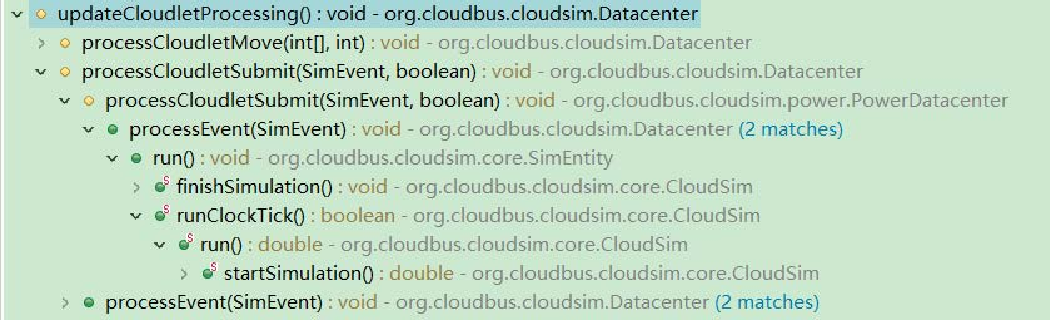
\includegraphics[width=1\textwidth]{./figures/2-updateCloudletProcessing.pdf}
	\caption{\label{fig:cloudletProcessing}Call hierarchy of function updateCloudletProcessing.}
\end{figure}

Figure 1 shows the call hierarchy of member function updateCloudletProcessing in class DataCenter. From this figure, we can figure out that the Cloudlet processing update process figure in the paper about CloudSim is wrong. Figure 2 is the fixed Cloudlet processing update process. At the end of the function updateCloudletProcessing, it will add a new VM\_DATACENTER\_EVENT to the future queue using function schedule. When we go back to the loop of Run function, the updateCloudletProcessing function will be triggered again.

\begin{figure}
	\centering
	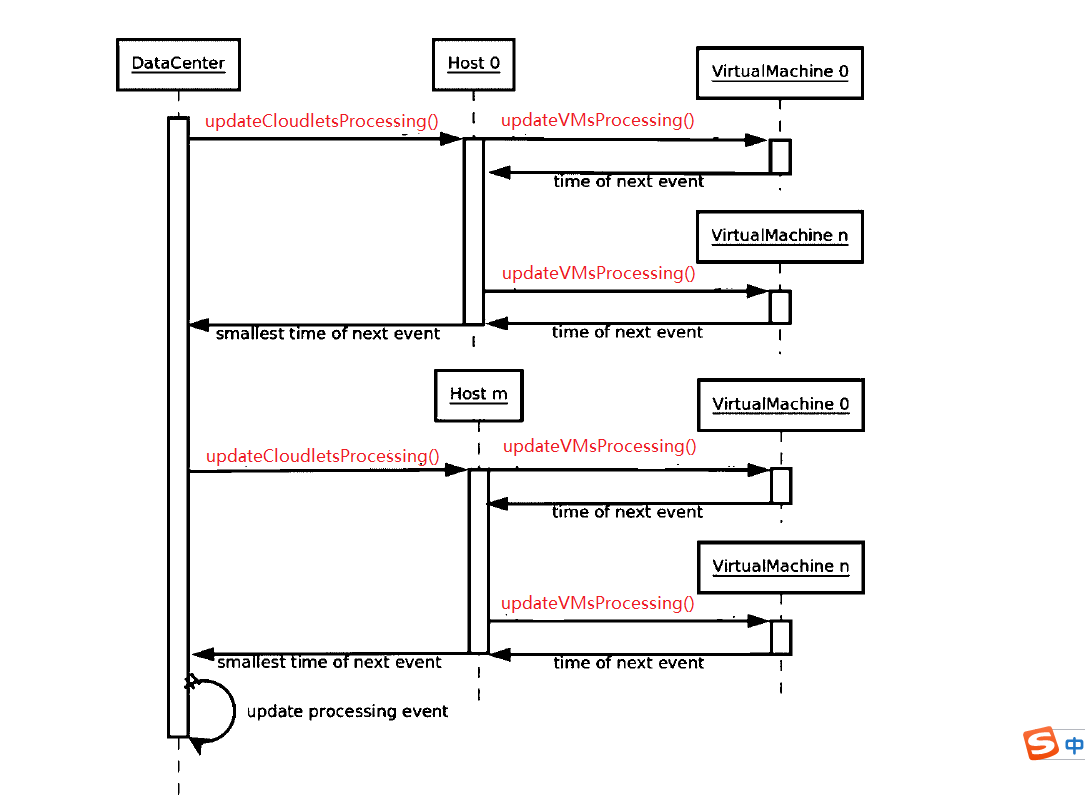
\includegraphics[width=1\textwidth]{./figures/3-processingSequence.png}
	\caption{\label{fig:processingSequence}Cloudlet processing update process.}
\end{figure}

\subsection{Simulation Framework of EdgeCloudSim}
\begin{figure}
	\centering
	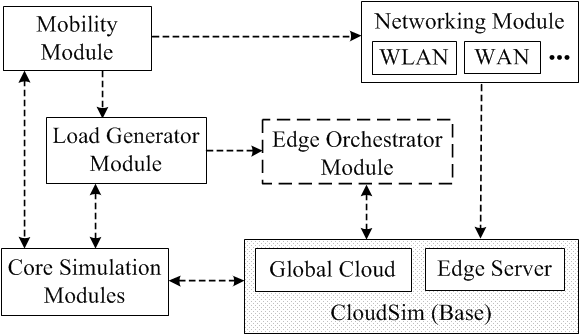
\includegraphics[width=1\textwidth]{./figures/1-edgecloudsim_diagram.png}
	\caption{\label{fig:frog}This is a figure caption.}
\end{figure}

As is shown in the picture1, there are two important classes in core package: ScenarioFactory and SimManager. The ScenarioFactory gets the parameters for the scenarios. And the SimManager receives the object of type ScenarioFactory. Moreover, the SimManager is a class extended from SimEntity class. The SimEntity is a class defined in CloudSim. And it has a function called startEntity(), which will schedule the task. 
\todo[inline, color=green!40]{Not sure if I can implement the task-based application here or change the schedule function in CloudSim}

\subsection{Modules in EdgeCloudsim}
\begin{enumerate}
	\item core: three are there important class in this module. ScenarioFactory.java is the class for factory scheme. SimManager.java class extends SimEntity class and it is related to CREATE\_TASK, CHECK\_ALL\_VM, GET\_LOAD\_LOG, PRINT\_PROGRESS, STOP\_SIMULATION. SimSettings.java is the class that stores all the configurations.
	\item cloud\_server: class CloudServerManager.java. This class actually just generate the hostlist, vmlist, local data center, and function to get the average utilization of all VMS. 
	\item edge\_server: class EdgeServerManager.java has similar functions as CloudServer.
	\item mobile\_processing: class MobileServerManager.java. This class enables the mobile devices have the ability to process task. We can also create data centers and virtual machines on it.
	\item edge\_client: MobileDeviceManager.java extends DatacenterBroker class in CloudSim. And it overwrite the processOtherEvent function and add new events: REQUEST\_RECEIVED\_BY\_CLOUD, REQUEST\_RECEIVED\_BY\_EDGE\_EDGE\_DEVICES.
\end{enumerate}


\subsection{Entities in EdgeCloudsim}
\begin{enumerate}
	\item SimManager: public class SimManager extends SimEntity
	\item MobileDeviceManager: public abstract class MobileDeviceManager  extends DatacenterBroker
	\item EdgeOrchestrator: public abstract class EdgeOrchestrator extends SimEntity
\end{enumerate}


\subsection{Relationship of Modules between CloudSim and EdgeCloudSim}
Because EdgeCloudSim is implemented on the top of CloudSim, it also relies on the discrete event management framework. 
MobileDeviceManager class extends DatacenterBroker class. So it implemented the following functions


\section{Design and Implementation}

\subsection{Scheduling in EdgeCloudSim}


\subsection{Task-based Application Design and Implementation}

\subsubsection{Task Lifecycle}
In EdgeCloudSim, task is atomic and cannot be divided into smaller tasks. Task-based application is an application which is composed by several smaller tasks. There may also have dependencies among these tasks. For instance, one sub-task can only starts after another sub-task. 

There are two ways to implemented tasked-based application feature in EdgeCloudSim. The first one is to change the code of CloudSim and add task-based features. The second one is to change the code of EdgeCloudSim and add the feature of tasked-based application.

We can define how to divide applications in XML file and store their dependencies.

The process of submit a task is as follows.


Figure 4 shows how generate the task list in LoadGenerator class.
\begin{figure}
	\centering
	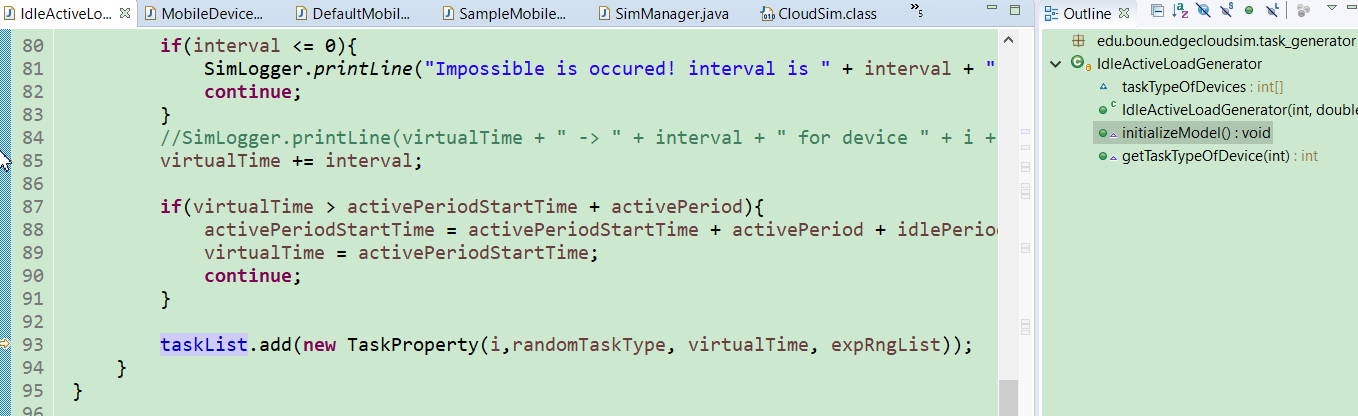
\includegraphics[width=1\textwidth]{./figures/Generate-task-LoadGenerator.png}
	\caption{\label{fig:frog}Generating Task List in LoadGenerator class.}
\end{figure}

Figure 5 shows how we submit the task using the schedule function.
\begin{figure}
	\centering
	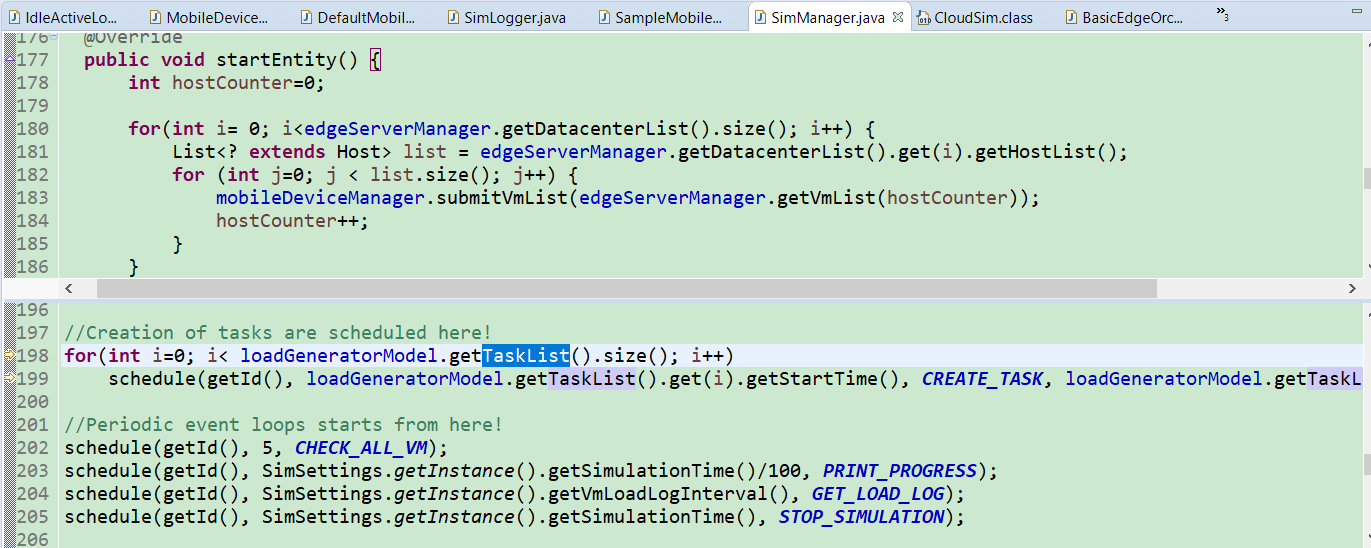
\includegraphics[width=1\textwidth]{./figures/schedule-submitTask.png}
	\caption{\label{fig:frog}Submit The Task Using the Schedule Function.}
\end{figure}


Figure 6 shows when we come to the clock tick in EdgeCloudSim, the event will be processed.
\begin{figure}
	\centering
	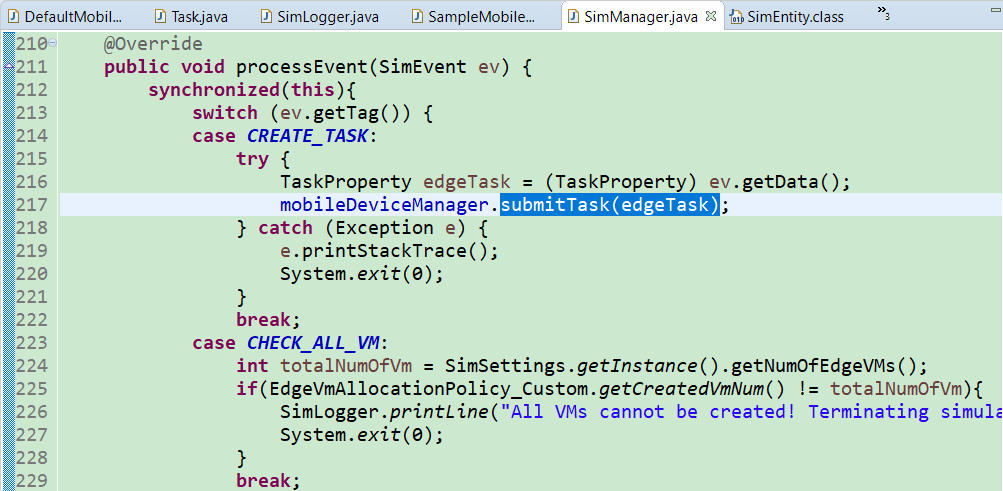
\includegraphics[width=1\textwidth]{./figures/5-SimManager-ProcessEvent-CREAT_TASK.png}
	\caption{\label{fig:frog}CREATE\_TASK event in in SimManager class.}
\end{figure}

Figure 7 shows the submitTask function in class MobileDeviceManager. MobileDeviceManager is extended from Broker. We can notice that the task created is added to log list in this class. The task is distinguished from other tasks by its CloudletId. 
\begin{figure}
	\centering
	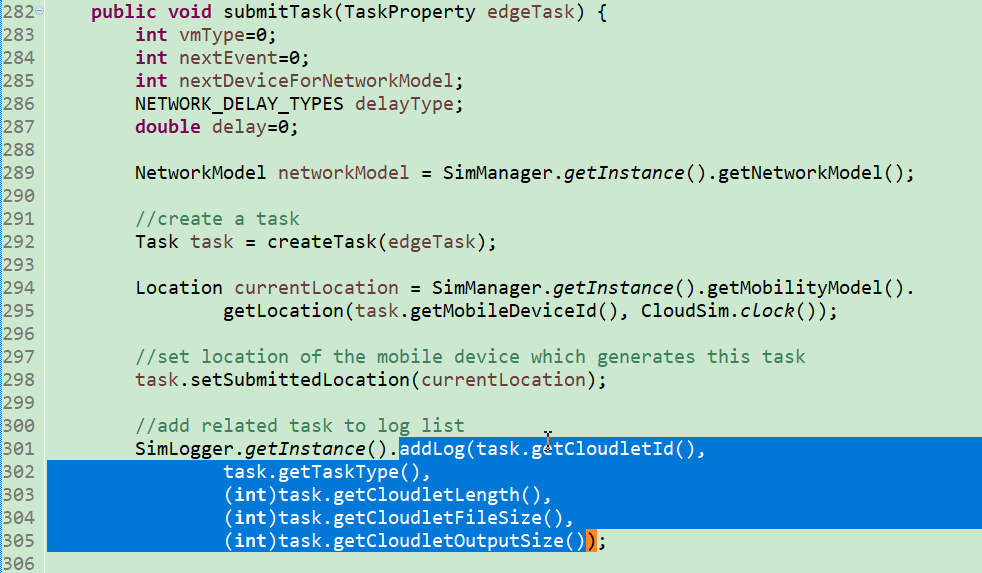
\includegraphics[width=1\textwidth]{./figures/4-submitTask-SampleMobileDeviceManager.png}
	\caption{\label{fig:frog}Task Submitted to the CloudSim Base in SampleMobileDeviceManager.java class.}
\end{figure}

Figure 8 what we do when the task finished. EdgeCloudSim will change the parameters concerning with execution time, the status in SimLogger class. Actually, we can submit new subtasks in this function. We can add a new field to Task.java class to determine whetehr the task is a subtask or an atomic task.
\begin{figure}
	\centering
	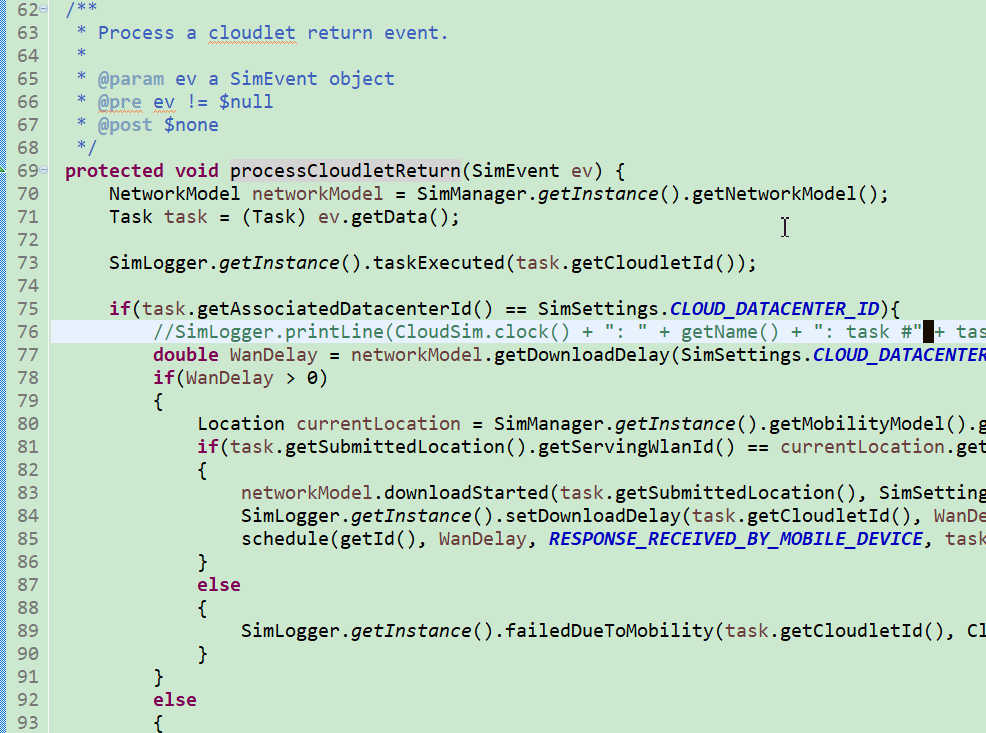
\includegraphics[width=1\textwidth]{./figures/processCloudletReturn.png}
	\caption{\label{fig:frog}ProcessCloudletReturn Function is Executed in MobileDeviceManager class.}
\end{figure}

 In the simulation, so we choose only submit a task to virtual machine when its dependencies has been met. In the SimManager class, the startEntity() function creates all the virtual machines in cloud server, edge server and mobile server. Besides, it also submits all the tasks to virtual machines. But in this project, we only submit the tasks whose dependencies has been met at this time. When a task is finished, it will send a CLOUDLET\_RETURN event to DatacenterBroker. In EdgeCloudSim, this event will be sent to MobileDeviceManager. Then processCloudletReturn function will be triggered. So when a task is finished, the tasks that have not been submitted will be checked. If there are tasks whose dependencies has been met now, it will be submitted to the VM at this time. The submit of tasks are based on the schedule function. We implement these functions in MobileDeviceManager class.

In processCloudletReturn function, it will test the execution place of the task, if it is executed in GENERIC\_EDGE\_DEVICE\_ID, the download delay will be added to the task, if it is executed in mobile device, the delay do not need to be add. We can test whether we need to submit new tasks to virtual machines at the  beginning of the function. 

\subsubsection{Task-based Application Design}
In this section introduces the design of task-based application based on EdgeCloudSim.

\subsubsection{Structure and Loading of Applications.xml}
The Applications.xml describes the types and parameters of applications in the simulation. Parameters in the original Applications.xml file of EdgeCloudSim is not explained, which makes it difficult to understand the meaning of these parameters. Figure 9 is an example of configurations of task-based applications. Figure 10 shows the original configurations of atomic applications.
The meanings of the parameters are listed as follows:

\begin{enumerate}
	\item usage\_percentage: The usage percentage here is used to decide the percentage of this type of application in all of the tasks generated. So add up usage\_percentage field in the applications.xml, we can get 100 because we have sumed up all the percentages of all applications.
	\item prob\_cloud\_selection: The probability that we choose the cloud to execute the task.
	\item poisson\_interarrival:
	\item active\_period: In active period, the edge devices can generate new tasks.
	\item idle\_period: In idle period, the edge devices can not generate new tasks.
\end{enumerate}

\begin{figure}
	\centering
	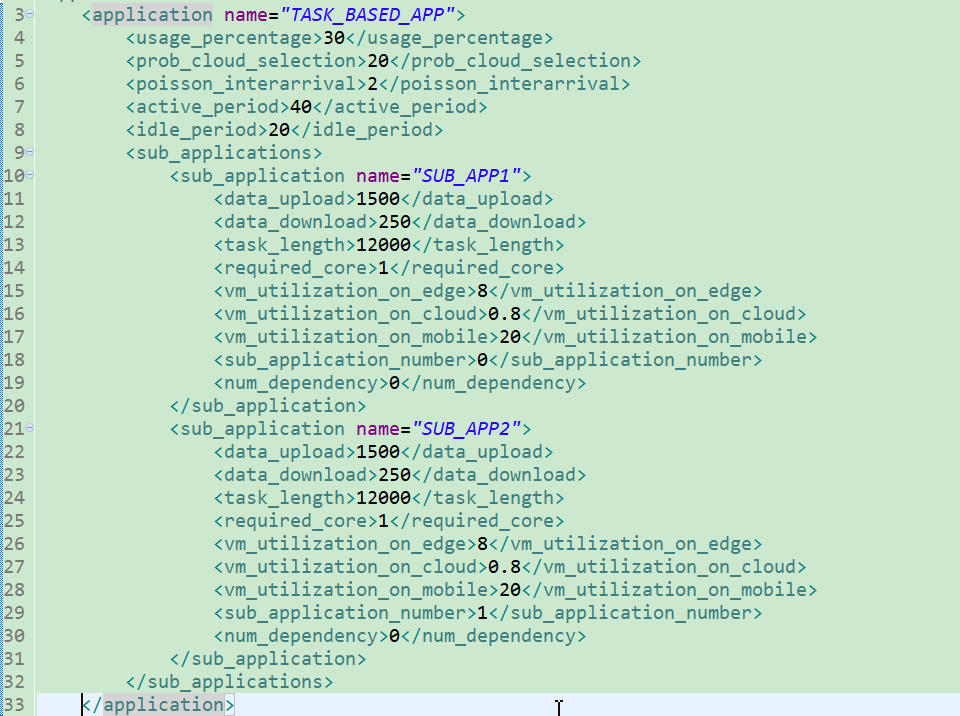
\includegraphics[width=1\textwidth]{./figures/task-based-xml.png}
	\caption{\label{fig:frog}Example of XML file of Task-based applications.}
\end{figure}

\begin{figure}
	\centering
	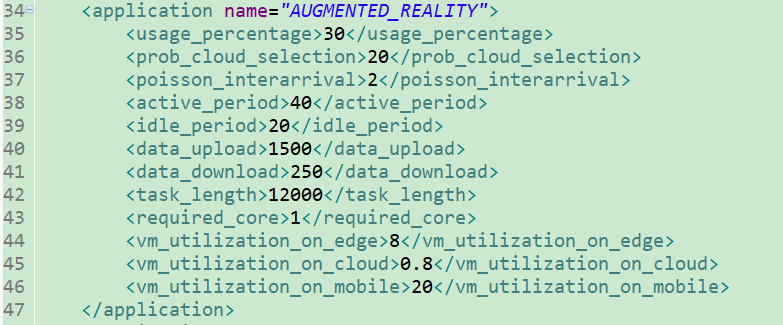
\includegraphics[width=1\textwidth]{./figures/atomic-application-xml.png}
	\caption{\label{fig:frog}Example of XML file of Atomic Applications.}
\end{figure}

The parameters are loaded in SimSettings.java. A new class called TaskBasedApplication.java is also implemented. The parameters of the applications and sub-applications are stored in the following two variables.

\begin{enumerate}
	\item private double[][] taskLookUpTable: store the parameters of applications.
	\item private double[][] subtaskLookUpTable: store the parameters of sub-applications.
	\item private TaskBasedApplication[] dependencyLookUpTable: store the dependency of each task-based application.
\end{enumerate}



\subsubsection{Sub-task Submission Using Topological Order}
In the class LoadGenerator, we generate the list properties of all tasks including all the sub tasks. The dependencies between all the sub-tasks are maintained in a list of objects of TaskBasedTask.java. The dependencies of them are maintained in this class. The reference of the LoadGenerator instance will be added to the instance of MobileDeviceManager. When MobileDeviceManager knows some tasks ends. It will check whether the task is a sub-task. If it is a sub-task. Then it will check whether there are other sub-tasks can be executed after the ending of this sub-task. If there are such tasks, the tasks will be send to datacenter using the function schedule.

\begin{figure}
	\centering
	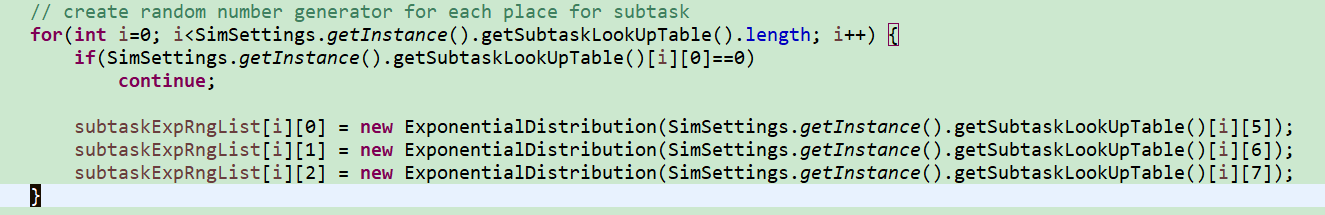
\includegraphics[width=1\textwidth]{./figures/y-1generator.png}
	\caption{\label{fig:frog}exponential number generator for sub-task.}
\end{figure}


The following picture shows how this project generate task properties for atomic task and bask-based task. After generating the random task type for edge devices, we judge whether it is a task-based task. If it is a task-based task, we will generate the properties of these sub-tasks.
\begin{figure}
	\centering
	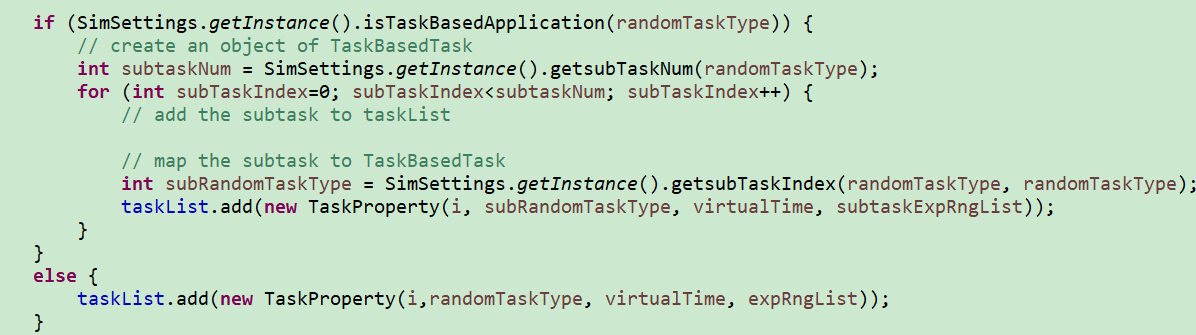
\includegraphics[width=1\textwidth]{./figures/y-2generator.png}
	\caption{\label{fig:frog}Generate task properties for atomic task and task-based task.}
\end{figure}

The dependencies of sub-task in task-based applications are handled in class TaskBasedApplication. This class can check the status of each task using two private variables called submitted and dependency. 

In this project, a class called TaskBasedTask.java is implemented to store the information of task-based task. This class can store the dependencies between each sub-tasks. We can trigger a function in the class to record the tasks that have finished. Moreover, it can calculate the sub-tasks that can be executed at this time. The object of TaskBasedTask will utilize the information stored in TaskBasedApplication to generate the dependencies of sub-tasks.


\subsubsection{Scheduling Algorithm in EdgeCloudSim}
Which module can we modify to achieve task-based application?
How to deal with task-dependency graph

\subsubsection{Component Diagram of the Simulation tool}
After adding the feature, the component diagram has changed.

\subsection{Task Migration}

\subsection{Probabilistic Network Failure Model}

\section{Experimental Results}
In this section, we did some experiment. We test the failure rate.

\section{Conclusions}


\section{Some \LaTeX{} Examples}
\label{sec:examples}

\subsection{Sections}

Use section and subsection commands to organize your document. \LaTeX{} handles all the formatting and numbering automatically. Use ref and label commands for cross-references.

\subsection{Comments}

Comments can be added to the margins of the document using the \todo{Here's a comment in the margin!} todo command, as shown in the example on the right. You can also add inline comments too:

\todo[inline, color=green!40]{This is an inline comment.}

\subsection{Tables and Figures}

Use the table and tabular commands for basic tables --- see Table~\ref{tab:widgets}, for example. You can upload a figure (JPEG, PNG or PDF) using the files menu. To include it in your document, use the includegraphics command as in the code for Figure~\ref{fig:frog} below.

% Commands to include a figure:
\begin{figure}
\centering
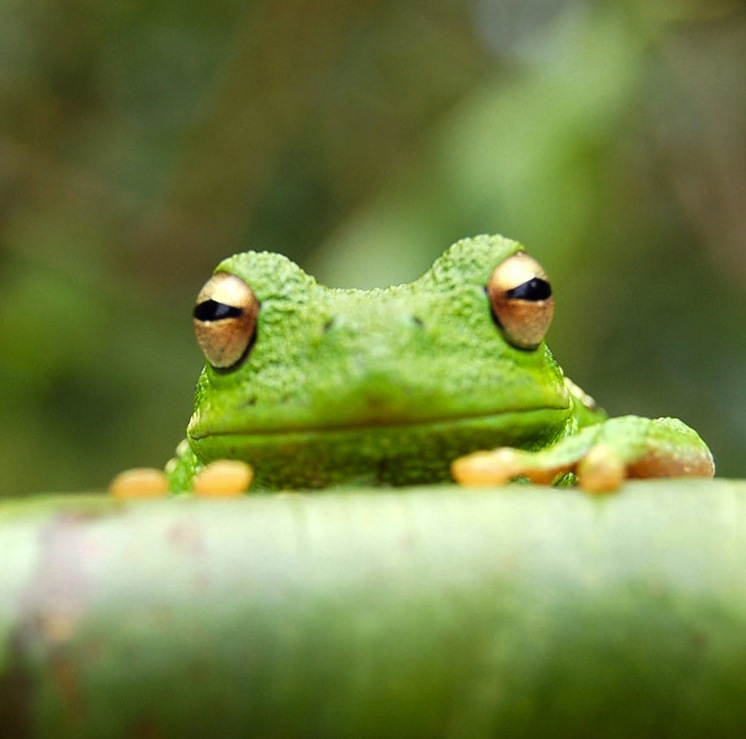
\includegraphics[width=0.5\textwidth]{frog.jpg}
\caption{\label{fig:frog}This is a figure caption.}
\end{figure}

\begin{table}
\centering
\begin{tabular}{l|r}
Item & Quantity \\\hline
Widgets & 42 \\
Gadgets & 13
\end{tabular}
\caption{\label{tab:widgets}An example table.}
\end{table}

\subsection{Mathematics}

\LaTeX{} is great at typesetting mathematics. Let $X_1, X_2, \ldots, X_n$ be a sequence of independent and identically distributed random variables with $\text{E}[X_i] = \mu$ and $\text{Var}[X_i] = \sigma^2 < \infty$, and let
$$S_n = \frac{X_1 + X_2 + \cdots + X_n}{n}
      = \frac{1}{n}\sum_{i}^{n} X_i$$
denote their mean. Then as $n$ approaches infinity, the random variables $\sqrt{n}(S_n - \mu)$ converge in distribution to a normal $\mathcal{N}(0, \sigma^2)$.

\subsection{Lists}

You can make lists with automatic numbering \dots

\begin{enumerate}
\item Like this,
\item and like this.
\end{enumerate}
\dots or bullet points \dots
\begin{itemize}
\item Like this,
\item and like this.
\end{itemize}

We hope you find write\LaTeX\ useful, and please let us know if you have any feedback using the help menu above.

\end{document}